\documentclass[10pt,twocolumn]{article} 

% required packages for Oxy Comps style
\usepackage{oxycomps} % the main oxycomps style file
\usepackage{times} % use Times as the default font
\usepackage[style=numeric,sorting=nyt]{biblatex} % format the bibliography nicely

\usepackage{amsfonts} % provides many math symbols/fonts
\usepackage{listings} % provides the lstlisting environment
\usepackage{amssymb} % provides many math symbols/fonts
\usepackage{graphicx} % allows insertion of grpahics
\usepackage{hyperref} % creates links within the page and to URLs
\usepackage{url} % formats URLs properly
\usepackage{verbatim} % provides the comment environment
\usepackage{xpatch} % used to patch \textcite
\usepackage{graphicx}

\addbibresource{references.bib}
\DeclareNameAlias{default}{last-first}

\xpatchbibmacro{textcite}
  {\printnames{labelname}}
  {\printnames{labelname} (\printfield{year})}
  {}
  {}

\pdfinfo{
    /Title (Computational Queries: Proof of Concept)
    /Author (Joaquín Madrid Larrañaga)
}

\title{Computational Queries: Proof of Concept}

\author{Joaquín Madrid Larrañaga}
\affiliation{Occidental College}
\email{jmadridlarra@oxy.edu}

\begin{document}

\maketitle

\section{Methods}
Since handtrack.js is a JavaScript based package made for web applications, it makes sense to create this installation using HTML5, CSS3, and a webcam - elements that are common with most computers.   Handtrack.js uses the video feed from a webcam to create a bounding box around each instance of a hand and face.  It also classifies each hand as ``open'', ``closed'', ``pinch'', or ``point''.  A tutorial by Larry Sass-Ainsworth on medium.com \cite{} provided a good starting point to get handtrack.js up and running.  This tutorial covered how to add handtrack.js to any HTML project and provided the source code for a functional, intuitive video feed that tracks face and hand positions. 

\begin{figure}[hbh]
\begin{center}
\scalebox{.4}{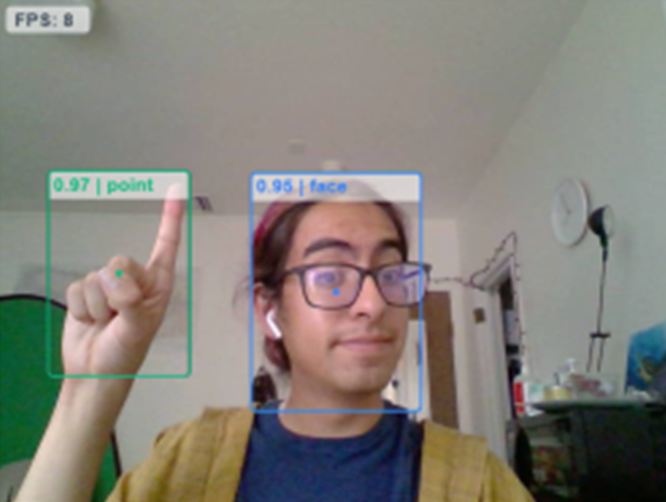
\includegraphics{images/bounding_example_resized.png}} 
\vspace{.5cm}
\caption{Classification and bounding boxes for a frame of a person}
\label{fig:bounding_boxes}
\end{center}
\end{figure}

After successfully installing handtrack.js, the JavaScript file was edited to use the JavaScript canvas feature to create a small circle instead of a bounding box that will be used to see hand movements for testing purposes (Figure \ref{fig:large_circle}). 

\begin{figure}[hbh]
\begin{center}
\scalebox{.4}{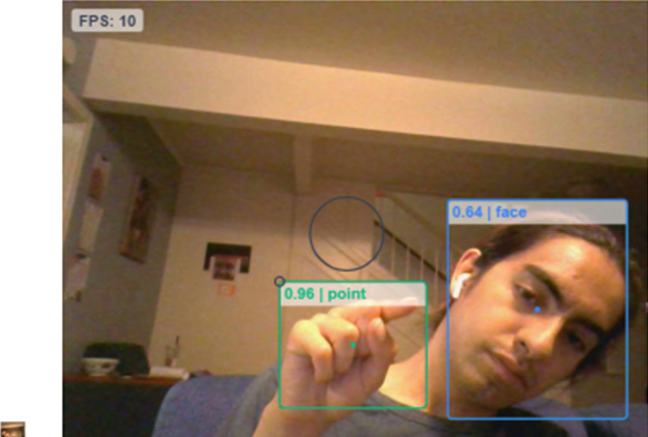
\includegraphics{images/big_circle_with_video.png}} 
\vspace{.5cm}
\caption{Adding the small circle cursor at the top left of the hand bounding box and the responsive large circle}
\label{fig:large_circle}
\end{center}
\end{figure}

Next, the live video feed was removed from the display so that only the small circles would be displayed. Then, the face recognition bounding box was filtered out so the small circle cursors only displayed when a hand was recognized in the frame.  Then, a responsive element was added. A large circle was placed at the center of the canvas using the JavaScript canvas capabilities (Figure \ref{fig:large_circle_no_vid}).  The file was then edited to move the large circle away from any small circles if they moved too close to the large circle.  In this way, the small circles would ``push'' the large circle around the canvas.  After testing this a couple of times, the code was tweaked so the large circle would stop moving at the edges of the canvas. Additionally, a button was added to ``reset'' the game by moving the large circle back to the center.  This is important because during the game testing the large circle would often get stuck in the corners of the canvas. This is likely because if the user tried to move their hand near the edge of the canvas, the computer would be unable to recognize their hand since it was cut off near the edge of the camera.  

\begin{figure}[hbh]
\begin{center}
\scalebox{.4}{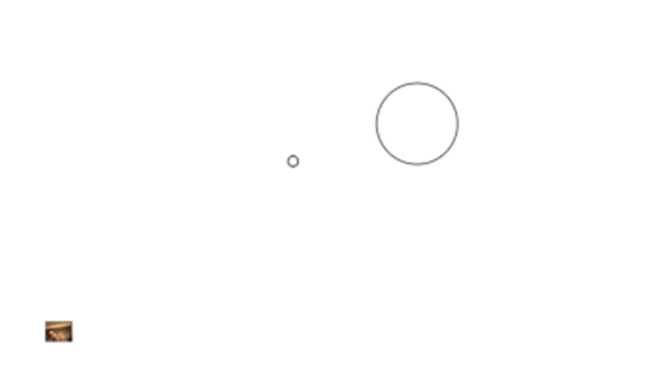
\includegraphics{images/big_circle_no_video.png}} 
\vspace{.5cm}
\caption{Removing live video output so only the small and large circles are displayed}
\label{fig:large_circle_no_vid}
\end{center}
\end{figure}



\section{Evaluation}
The evaluation metric for this project relies heavily on qualitative observations.  It is qualitatively clear that the program identifies hands well. This means that the program rarely fails to display a bounding box when a hand is present and never displays extraneous bounding boxes.  Furthermore, there is an additional feature that classifies the hand position as one of the following: closed (as in a fist), open (as in a high five), point (as in one finger up), and pinch (unclear).  After a qualitative investigation, it is clear that this classification does very well at identifying open and closed hands correctly, but also identifies pointed and pinched hands as closed.   During the entire testing and creation process, the program only classified a hand as ``pinch'' four times... and two were incorrect classifications. As a result, it is unclear what ``pinch'' means and what constitutes a ``pinched'' hand since active attempts to produce a classification of ``pinch'' were catergorized incorrectly as ``closed''.  

Despite imperfect hand classification, this program has a qualitative success rate of 100\% for classifying faces.  It accurately created a bounding box for for the researcher's face every time the program was turned on. 

While the program does create bounding boxes for hands and faces well, it has trouble with overlapping bounding boxes.  When placing both hands together, the program often fails to recognize either hand. Furthermore, when a user's hand crosses their face, the program loses the bounding box on the hand and only displays the bounding box on the face, even though the hand is in front of the face. As a result, the current implementation of the software does not create a small circle cursor when someone's hand is in front of their face because the program is unable to recognize the hand and create a bounding box. In addition, the program makes no distinction between left and right hands (nor if the hand is facing front or back).  These issues are potentially problematic and will be discussed further. 

\section{Discussion}
It is important to mention that the ``point'' classification does not distinguish where in the bounding box the outstretched finger is pointing towards. It only checks to see if one finger is outstretched.  Pointing with any of the five fingers on the hand produces a ``point'' classification. However, this is potentially problematic for fine tuned interaction.  Since handtrack.js only creates a bounding box around the hand and does not distinguish where exactly the pointed finger is pointing, the small circle cursor will be based on the bounding box and not the finger that is pointing. This means that the cursor will always be correct relative to the hand movement, but not exactly correct with regards to the actually pointing finger. As a result, the next iteration of the code will likely assume that hands on the left side of the screen will be left hands (thus the pointer finger is on the right side of the hand).  And vice versa.  Therefore, the small circle cursor will be on the right side of the bounding box. However, this approach may become an issue if multiple users interact with the installation at once. 

During the testing of the above code, it became clear that Handtrack.js has a very slow frames per second speed that fluctuates. 
The current model displays the frames per second (FPS) of the video output.  This output fluctuates based on how fast the recognition software can process each frame of the video input. More processing time = less frames outputted.  Fortunately, this is not a sequential delay in output (the cause of lag, also called first in, first out), but rather a first in, first out approach.  In this way, any frames that were missed as a result of the processing time are discarded and the next newest frame is processed.  Even though this approach does not interfere with continuity for the viewer, it produces a jerky video as a result of the reduction in frames per second.  

The industry standard for high definition films is 24 frames per second \cite{} which is the smallest number of FPS that creates smooth motion.  The current model moves between 8FPS and 16FPS. While this produces a jerky live video feed, the individual bounding boxes create convincing continuous motion when the live video feed is removed and only the bounding boxes (replaced by small circles) remain. Unfortunately, this motion needs to be fairly slow on the part of the user.  Since faster motion causes motion blur in photos, each individual frame will be blurred if the user moves quickly. As a result, the image recognition software is unable to correctly identify the bounding boxes of the hands since their shape is blurred. Further research suggests that an easy solution is to reduce the exposure time for each individual frame which will remove the blur \cite{} and allow for better hand recognition.   

Overall, handtrack.js will be a useful tool for the interactive art installation, though it may not be the best tool.  Further research revealed a tool called handsfree.js which tracks individual finger and limbs as well as hands and faces for the purpose of interacting with a computer through movement.  Further research should investigate the differences between handtrack.js and handsfree.js in functionality, accuracy, and appropriateness for the project.  

As a whole, this project serves as proof of concept for a larger interactive art installation that takes user movement as an input. By creating a webapp that has users move their hands to push a circle around the screen, the concept of a movement controlled experience is proven.  However, in the final project, the large circle will be replaced with geometric shapes that respond in other ways than moving around the canvas. In this way, this simple webapp has successfully proven the feasibility of ``Computational Queries,'' an interactive art installation that seeks to explore curosity and discoverability. 


\printbibliography 

\end{document}
